37. \begin{figure}[ht!]
\center{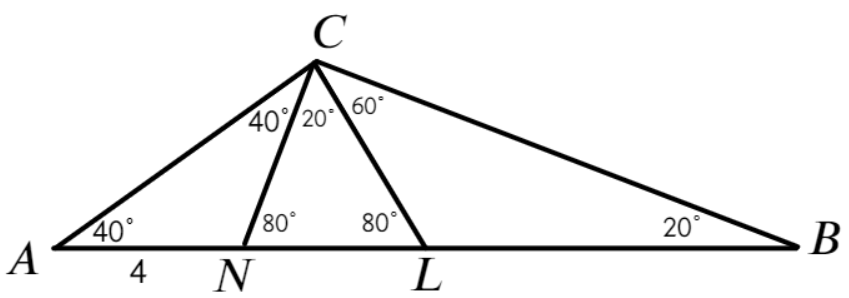
\includegraphics[scale=0.35]{g37.png}}
\end{figure}\\
Пусть $CL$ --- биссектриса. Сделаем дополнительное построение: отметим на стороне $AB$ точку $N$ так, чтобы $BC=BN.$ Тогда $AN=AB-BN=AB-BC=4.$ Треугольник $CBN$ является равнобедренным с углом при вершине $20^\circ,$ значит $\angle CNB=\angle NCB=(180^\circ-20^\circ):2=80^\circ.$ Угол $C$ равен $180^\circ-20^\circ-40^\circ=120^\circ,$ значит $\angle LCB=120^\circ:2=60^\circ,\ \angle NCL=80^\circ-60^\circ=20^\circ,\ \angle ACN=60^\circ-20^\circ=40^\circ,\ \angle CLN=180^\circ-20^\circ-80^\circ=80^\circ.$ Таким образом, треугольники $ACN$ и $NCL$ являются равнобедренными, а поэтому $CL=CN=AN=4.$\\
